% Post-P&R floorplan diagram (Fig. 3) — clean TikZ rendering driven by
% bounding boxes extracted from soc_top.def by extract_floorplan.py.
% Build: cd paper/figures/src && pdflatex fig3_layout.tex && mv fig3_layout.pdf ../
\documentclass[border=2pt]{standalone}
\usepackage{mathptmx}
\usepackage{tikz}
\usetikzlibrary{calc,backgrounds}

\definecolor{navy}{HTML}{1F3A5F}
\definecolor{navylight}{HTML}{D6DEEC}
\definecolor{tlgred}{HTML}{A83232}
\definecolor{redfill}{HTML}{F5DCDC}
\definecolor{stdgray}{HTML}{F2F2F2}

\begin{document}
% TikZ x-coordinate corresponds to µm × scale; we scale 1 µm = 0.05mm
% so the 1500 µm die spans 75 mm. With column width ≈ 86 mm, this
% leaves ~5 mm margin on each side.
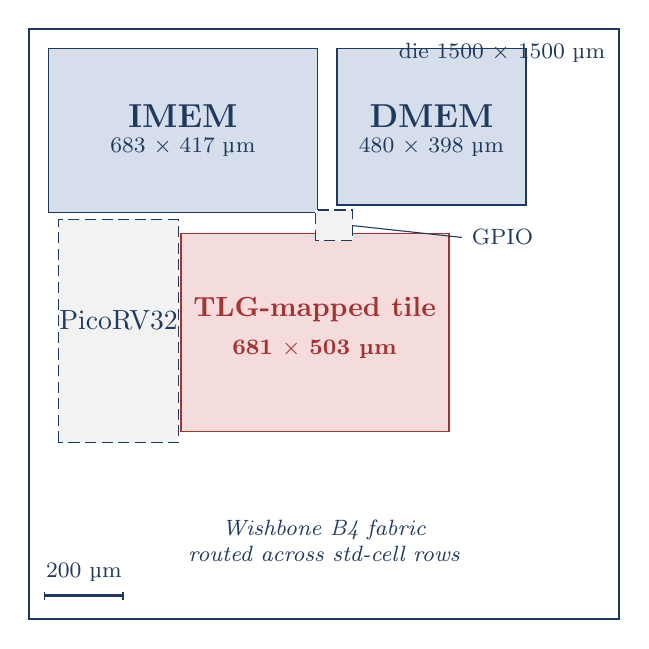
\begin{tikzpicture}[
    x=0.05mm, y=0.05mm,
    font=\rmfamily,
    line width=0.6pt,
    every node/.style={font=\rmfamily},
  ]

  % ---------- Die outline -------------------------------------------------
  \draw[draw=navy, line width=0.8pt] (0,0) rectangle (1500,1500);

  % ---------- Memory macros (top region) ----------------------------------
  % IMEM: (50, 1033.46) -> (733.10, 1450)  size 683.10 x 416.54
  \fill[navylight] (50, 1033.46) rectangle (733.10, 1450);
  \draw[draw=navy, line width=0.6pt] (50, 1033.46) rectangle (733.10, 1450);
  \node[anchor=center, navy, font=\rmfamily\bfseries\large]
    at (391.55, 1278) {IMEM};
  \node[anchor=center, navy, font=\rmfamily\footnotesize]
    at (391.55, 1198) {683 $\times$ 417 \textmu m};

  % DMEM: (783.10, 1052.50) -> (1262.88, 1450)  size 479.78 x 397.50
  \fill[navylight] (783.10, 1052.50) rectangle (1262.88, 1450);
  \draw[draw=navy, line width=0.6pt] (783.10, 1052.50) rectangle (1262.88, 1450);
  \node[anchor=center, navy, font=\rmfamily\bfseries\large]
    at (1022.99, 1278) {DMEM};
  \node[anchor=center, navy, font=\rmfamily\footnotesize]
    at (1022.99, 1198) {480 $\times$ 398 \textmu m};

  % ---------- Std-cell modules (extracted from DEF, 5-95 percentile) ------
  % u_tile (TLG-mapped tile, RED HIGHLIGHT, dominant block)
  % core_bbox (386.08, 477.44) -> (1067.06, 988.64). Trim down to 980 to
  % avoid bumping into the macro region.
  \fill[redfill] (386, 477) rectangle (1067, 980);
  \draw[draw=tlgred, line width=0.7pt] (386, 477) rectangle (1067, 980);
  \node[anchor=center, tlgred, font=\rmfamily\bfseries\normalsize, align=center]
    at (726, 740) {TLG-mapped tile\\[0.4ex]
      \rmfamily\footnotesize 681 $\times$ 503 \textmu m};

  % u_cpu (PicoRV32) — interleaves with u_tile in 386-543 range; visualize
  % only the non-overlapping LEFT region for clarity.
  \fill[stdgray] (76, 449) rectangle (380, 1015);
  \draw[draw=navy, line width=0.5pt, dash pattern=on 4pt off 2pt]
    (76, 449) rectangle (380, 1015);
  \node[anchor=center, navy, font=\rmfamily\normalsize, align=center]
    at (228, 760) {PicoRV32};

  % u_gpio (top-right of std-cell zone, near macros)
  % core_bbox (728, 962) -> (823, 1081); trim ymax so it stays below DMEM.
  \fill[stdgray] (728, 962) rectangle (823, 1040);
  \draw[draw=navy, line width=0.5pt, dash pattern=on 4pt off 2pt]
    (728, 962) rectangle (823, 1040);
  % GPIO label outside the small box, with leader line
  \node[anchor=west, navy, font=\rmfamily\footnotesize] (gpiolabel)
    at (1100, 970) {GPIO};
  \draw[draw=navy, line width=0.4pt] (823, 1000) -- (gpiolabel.west);

  % ---------- Wishbone fabric annotation (no extracted bbox; flattened) ---
  % Place the italic annotation in the empty bottom portion of the die.
  \node[anchor=center, navy, font=\rmfamily\itshape\footnotesize, align=center]
    at (750, 200) {Wishbone B4 fabric\\
      routed across std-cell rows};

  % ---------- Die-size annotation (top-right corner) ----------------------
  \node[anchor=north east, navy, font=\rmfamily\footnotesize]
    at (1490, 1490) {die 1500 $\times$ 1500 \textmu m};

  % ---------- Scale bar (bottom-left) -------------------------------------
  \draw[draw=navy, line width=1.0pt] (40, 60) -- (240, 60);
  \draw[draw=navy, line width=0.6pt] (40, 50) -- (40, 70);
  \draw[draw=navy, line width=0.6pt] (240, 50) -- (240, 70);
  \node[anchor=south, navy, font=\rmfamily\footnotesize]
    at (140, 70) {200 \textmu m};

\end{tikzpicture}
\end{document}
